\documentclass{article}
\usepackage[a4paper, margin=3cm]{geometry}
\usepackage[utf8]{inputenc}
\usepackage[hungarian]{babel}
\usepackage{t1enc}
\usepackage{todonotes}
\usepackage{amsmath}
\usepackage{amssymb}
\usepackage{booktabs}
\usepackage{url}
\usepackage{tikz}
\usepackage{hyperref}
\usepackage{listings}
\usepackage{upquote}
\usepackage{biblatex}
\usepackage{csquotes}
\usepackage{amsthm}

% Tikz styles
\usetikzlibrary{arrows.meta, positioning}
\tikzstyle{box} = [rectangle, draw=black, text centered, minimum height=1cm, align=center]
\tikzstyle{inputbox} = [box, fill=red!20, minimum width=2cm]
\tikzstyle{process} = [box, fill=yellow!40, minimum width=3.5cm, rounded corners]
\tikzstyle{outputbox} = [box, fill=green!20, minimum width=3cm]
\tikzstyle{arrow} = [thick, ->, >=Stealth]

\title{Hogyan parkol egy önvezető autó?}
\author{Szente Péter}
\date{2025. július}

\addbibresource{elteiktdk.bib}


\begin{document}

\maketitle

\section{Motiváció}
Az önvezető és vezetést segítő rendszerek az autóipar egyik vezető trendjévé váltak. Segítségükkel az autók biztonságosabbak lesznek, kevesebb energiát használnak, vagy kényelmi funkciókkal bővülnek. A korai vezetést segítő rendszerek fókusza a biztonság és a kényelem volt. Ilyenek például a blokkolásgátló rendszer, a sávtartás és a sebességtartás, illetve vészfékezés funkció, mely a frontális ütközést hivatott elkerülni az autó lelassításával. Az utóbbi években egyre több autót szerelnek fel nagy felbontású szenzorokkal (lidar, radar, kamera), melyek feltérképezik a jármű környezetét. Az önvezető funkciók feladata a rendelkezésre álló információk alapján a vezető inputjának hatására egy biztonságos manőver megtervezése és végrehajtása.


\section{Modellek}

% fizikai modell
Az útvonaltervezés az algoritmikus megoldások mellett már a kezdetektől fogva erősen támaszkodik fizikai és matematikai eredményekre. Mivel a cél egy fizikai korlátokkal rendelkező jármű navigálása, így fontos a \textit{jármű modellezése}. Az egyik leggyakrabban alkalmazott modell az \citeauthor{ackermann1990robust} modell \cite{ackermann1990robust}. Ez feltételezi, hogy a kerekek a differenciálhajtóműnek köszönhetően csúszásmentesen haladnak. Az egy tengelyen lévő kerekeket további egyszerűsítésként gyakran egynek veszik. Ekkor biciklimodellről \cite{polack2017kinematicBicycleModel} beszélünk. Ezen egyszerűsítések jól modellezik egy négykerekű jármű mozgását, ha a sebesség nem túl nagy. \citeauthor{polack2017kinematicBicycleModel} azonban rámutatnak \cite{polack2017kinematicBicycleModel}, hogy bár az útvonaltervezésben ezzel a modellel követhető útvonalat kapunk, a kontrollerben már nem érdemes használni, mert az apró hibák a manőver végrehajtása során összeadódnak, és a jármű letér a tervezett útvonalról.

% Freespace
Egy másik fontos modell az autó optimális hosszúságú útvonalát adja meg abban az esetben, ha nincsenek akadályok. Ezen \textit{szabadtéri útvonaltervezés} megoldását \citeauthor{dubins1957curves} írta le először \cite{dubins1957curves} azzal a megkötéssel, hogy a jármű csak előre mehet. Fontos eredmény, hogy az optimális útvonal legfeljebb 3 útvonaldarabból áll, melyek egyenesek vagy adott sugarú körívek lehetnek. Ez lehetővé teszi, hogy a legrövidebb útvonalat egyszerű matematikai formulák segítségével kiszámítsuk. A teljes probléma megoldását \citeauthor{reeds1990optimal} adták meg \cite{reeds1990optimal}. Az előzőhöz hasonló eredmény szerint az optimális útvonal legfeljebb 5 útvonaldarabból áll, melyek között legfeljebb 2 menetirányváltás is lehet.

% Precepció
Egy önvezető járműnél a környezet érzékelésére, a \textit{percepcióra} széles szakirodalom elérhető. \citeauthor{yeong2021sensorFusion} egy viszonylag friss összefoglaló tanulmányban \cite{yeong2021sensorFusion} összefoglalják a használt módszereket. A percepciós rendszer alapvetően szenzorok kombinációjából áll, mint például LIDAR, radar, kamerák és ultrahangos érzékelők. A szenzorok segítségével a jármű képes felismerni a környezetében található akadályokat, a szabad parkolóhelyeket és az útfelület geometriáját. A szenzoros adatok összeolvasztásával (sensor fusion) pontos és megbízható környezetérzékelést próbálnak megvalósítani.\footnote{~A percepcióval a dolgozat nem foglalkozik részletesen.} Az útvonaltervezés a szenzorfúzió komponens kimenete alapján tervezi az útvonalat, így fontos ezen lépés megbízhatósága.

% Geometria
Az akadályok elkerülésére különböző \textit{geometriai} megközelítéseket alkalmaznak. Itt megkülönböztethetünk poligon alapú és mező alapú módszereket. A poligon alapú módszerek \cite[7--8.~fejezet]{preparata2012computationalGeometry} leginkább egy útvonal vagy pozíció ellenőrzésére alkalmasak. Általában bináris kimenetükből az derül ki, ütközik-e az útvonal. 

A \textit{mező alapú} módszerek optimalizációs feladatok megoldására alkalmasak. Az legismertebb mező alapú módszer a Voronoi-diagram alapú akadályelkerülés, amely a jármű akadályoktól való távolságát próbálja maximalizálni az útvonal minimalizálása mellett. Egy másik gyakran alkalmazott megoldás a potenciálmező-alapú megközelítés \cite{tanzmeister2014efficientCollisionField, ziegler2010fastOccupancyGrid}, amely egy vektormezőt hoz létre a jármű mozgásának irányítására, elkerülve az akadályokat és vezetve a cél felé. 

% A*, RRT*
Az \textit{útvonaltervezés} feladata ezen építőelemekből a kritériumoknak megfelelő útvonal elkészítése. Az algoritmusokat osztályozhatjuk keresés alapú és felfedezés alapú algoritmusokra \cite{gonzalez2015review}. A keresés alapú algoritmusok közül a legismertebb a hibrid A* \cite{dolgov2008hybridAstar} és variánsai. Ezek az algoritmusok a keresési térben egy heurisztika segítségével keresik meg az optimális útvonalat. A felfedezés alapú algoritmusok közül a legismertebbek az RRT-variánsok\footnote{~Rapidly Exploring Random Trees} \cite{noreen2016RRTsurvey}. Ezek az algoritmusok először véletlen lépésekkel felfedezik a keresési teret. Ha találnak megoldást, akkor utána azt több iteráción keresztül finomítják.

% Geometriai simítási eljárások
A tervezett útvonal görbülete gyakran tartalmaz szakadásokat \cite{zhang2021jpsBézier}, melyeket valamilyen \textit{simítási eljárással} \cite{gonzalez2015review} javíthatunk. Gyakran használnak Bézier-görbéket \cite{zhang2021jpsBézier} és spline interpolációt \cite{berglund2009bSplinePaths} sima útvonalak meghatározására. Mindkettőnél kihívás a görbület korlátozása \cite{maekawa2010curvatureContBSpline, cimurs2017bezierSmoothingCurvature}. Ha a görbület egy intervallumon nagyobb, mint a maximális görbület vagy szakadási helye van, akkor a jármű letér a meghatározott pályáról. Vannak olyan görbék, melyek természetesen követik a kormányzás által meghatározott trajektóriát. A \textit{klotoidok} \cite{brezak2013clothoidApprox} a görbület állandó sebességű változását feltételezik, így ideális illesztőgörbék az útvonaltervezés számára.

% Optimalizációs módszerek
Még ha az útvonaltervező algoritmus a hosszban optimálishoz közeli és követhető utat ad, akkor is éremes tovább javítani rajta \cite{dolgov2008hybridAstar}. Az útvonal gyakran tartalmaz felesleges kormányzásokat. Ezeket egy \textit{lokális optimalizációs} eljárással kisimíthatjuk. Itt figyelembe kell venni a maximális megengedett görbületet és az objektumoktól vett távolságot is.

% Kontroll
Legvégül az elkészült útvonalat az autónak végig kell követnie. Ezt a \textit{kontroller} végzi a motor és a kormánymotor állapotának változtatásával a tervezett trajektória alapján. Itt ismét fontos szerepet játszik a fizikai modell és a bizonytalansági tényezők figyelembe vétele. \citeauthor{liu2023controlSurvey} egy 2023-as tanulmányukban \cite{liu2023controlSurvey} részletesen bemutatják a probléma komplexitását. Habár a kontroll az információs láncban az útvonaltervezés után van, mégis erős kimeneti követelményeket támaszt a tervezéssel szemben.

\begin{figure}
  \centering
  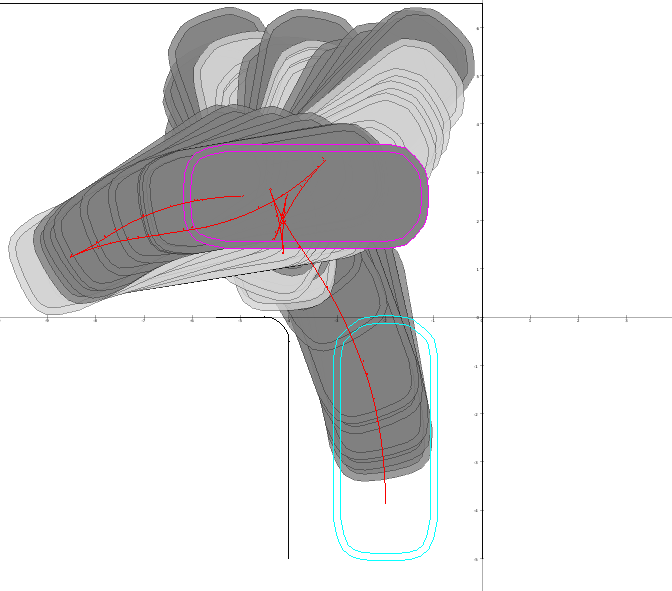
\includegraphics[width=0.75\linewidth]{images/scenes/cross-blocked.png}
  \caption[Egy kihívást jelentő parkolási eset]{Egy kihívást jelentő parkolási esethez, a blokkolt merőleges parkoláshoz tervezett útvonal $6$ irányváltással}
  \label{fig:opening-cross-blocked}
\end{figure}

\section{Mit nevezünk útvonaltervezésnek?}
% Útvonaltervezés definíciója
A \textit{kinematikai útvonaltervezés} során a cél számítási módszerek alkalmazásával két térbeli konfiguráció közötti folytonos útvonal meghatározása az összes fizikai korlát betartása és az akadályok elkerülése mellett.

Ez egy tisztán geometriai probléma, amely mellőzi az időbeli és dinamikai komplexitást. Önvezető járműveknél ezt általában nem tehetjük meg, azonban ha feltesszük, hogy a jármű alacsony sebesség mellett hajtja végre a manővereket, akkor a feltételezéseink jól modellezik a valóságot \cite{polack2017kinematicBicycleModel}. Ezt az egyszerűsítést elfogadjuk, hiszen a dolgozat fő fókusza a parkolás. Ebben az esetben körültekintően kell navigálni a sok akadály és a rossz láthatóság, pontosabban az objektumok takarása miatt.

% Elhelyezés az önvezetés komponens diagrammjában, hatáskör meghatározása
A probléma megoldásához fontos elkülönítenünk az útvonaltervező komponens hatáskörét. Ezt szemlélteti \aref{fig:what-is-motion-planning}. ábra. Az útvonaltervezésnek nem része a szenzoradatok feldolgozása és címkézése. Ezt a percepció komponens végzi, melynek része a szenzorfúziós hely- és helyzetmeghatározás is. A percepció kimenete a környezetben található \textit{objektumok} járműhöz viszonyított relatív pozíciója és az objektumok fajtája. Ezek tipikusan lehetnek alacsony objektumok (pl. fekvőrendőr, útburkolati jelek), melyek felett áthajthatunk, és magas objektumok, melyeket mindenképp ki kell kerülnünk. A későbbiekben csak a magas objektumokkal foglalkozunk és \textit{akadályoknak} hívjuk őket.

\begin{figure}[ht]
\centering
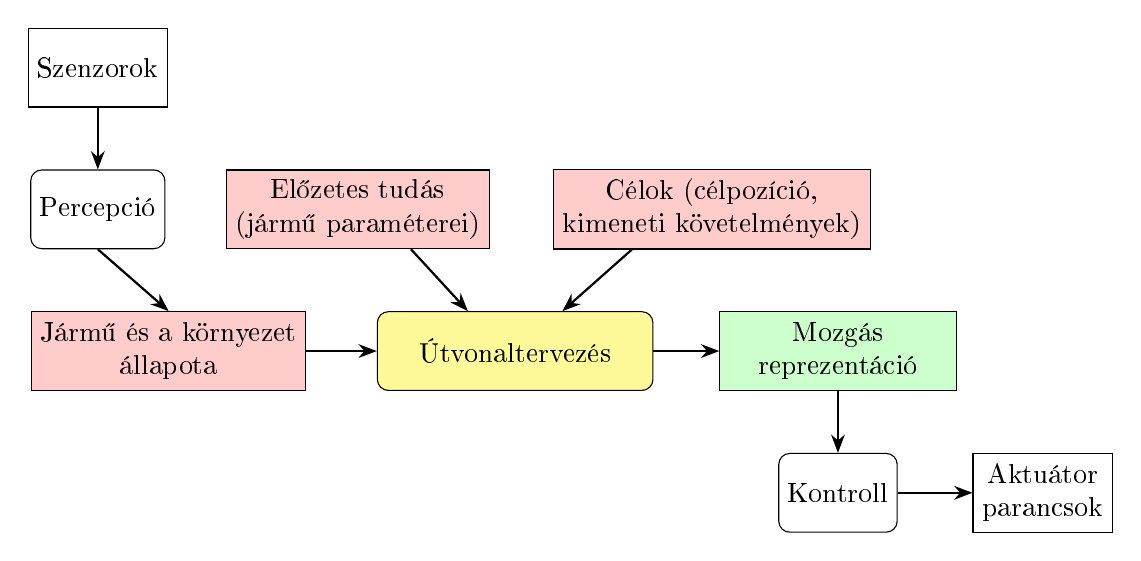
\begin{tikzpicture}[node distance=1.8cm]
  % Tervezés
  \node (planning) [process] {Útvonaltervezés};
  % Globális input
  \node (prior) [inputbox, above of=planning, xshift=-2cm] {Előzetes tudás\\(jármű paraméterei)};
  \node (objectives) [inputbox, above of=planning, xshift=2.5cm] {Célok (célpozíció,\\kimeneti követelmények)};
  % Környezeti input
  \node (state) [inputbox, left of=planning, xshift=-2.6cm] {Jármű és a környezet\\állapota};
  \node (perception) [box, left of=prior, xshift=-1.5cm, rounded corners] {Percepció};
  \node (sensors) [box, above of=perception] {Szenzorok};
  % Kimenet
  \node (motion) [outputbox, right of=planning, xshift=2.3cm] {Mozgás\\reprezentáció};
  % Kontoll
  \node (control) [box, below of=motion, rounded corners] {Kontroll};
  \node (actuator) [box, right of=control, xshift=.8cm] {Aktuátor\\parancsok};
  % Nyilak
  \draw [arrow] ([xshift=-1cm]prior.south east) -- ([xshift=-0.6cm]planning.north);
  \draw [arrow] ([xshift=1cm]objectives.south west) -- ([xshift=0.6cm]planning.north);
  \draw [arrow] (state.east) -- (planning.west);
  \draw [arrow] (planning.east) -- (motion.west);
  \draw [arrow] (perception.south) -- (state.north);
  \draw [arrow] (sensors.south) -- (perception.north);
  \draw [arrow] (motion.south) -- (control.north);
  \draw [arrow] (control.east) -- (actuator.west);
\end{tikzpicture}
\caption[Önvezetés komponensdiagrammja]{Önvezetés komponensdiagrammja\footnotemark}
\label{fig:what-is-motion-planning}
\end{figure}
\footnotetext{Leegyszerűsített modell \href{https://motion.cs.illinois.edu/RoboticSystems/WhatIsMotionPlanning.html}{Kris Hauser vizualizációja} alapján.}

Az útvonaltervező ismeri továbbá a jármű paramétereit. Ezek közül az egyik legfontosabb a jármű \textit{kontúrja} (felülnézeti, kétdimenziós körvonala). A másik legfontosabb paraméter a legszűkebb kanyarodási manőver, amit végre tudunk hajtani. Ez utóbbi a kinematikai modellből származó számunkra legfontosabb paraméter.

Az útvonaltervezés egy költséges művelet, így mindig egy jól definiált céllal hajtjuk végre. Ez tipikusan egy útvonal megtalálása a jelenlegi vagy egy prediktált kezdőpozícióból egy célpozícióba. A célok között lehetnek megkötések is. Ezek gyakran a menetirányra vagy az útvonal simaságára vonatkoznak.\footnote{~Például, ha a jármű előre mozgásban van, akkor az útvonal nem kezdődhet hátramenettel. Egy másik gyakori feladatban arra vagyunk kíváncsiak, elérhető-e a célpozíció egy egyszerű manőverrel. Ilyenkor az útvonal egyáltalán nem tartalmazhat hátramenetet.}

Az útvonaltervező valamilyen útvonal-reprezentációt állít elő, mely összeköti a kiindulási- és a célpozíciót. Ezt aztán a kontroller hajtja végre. Ezen modul feladata a trajektória lekövetése a jármű aktuátorainak aktiválásával, és a kisebb hibák korrigálása. A kontroller nem fog tudni bármilyen útvonalat lekövetni, így fontos, hogy a tervezett útvonal \textit{vezethető} legyen. Ezen kimeneti követelményt általában az útvonal bizonyos szintű simaságával és folytonosságával formalizáljuk.

\section{A jármű kinematikai modellje}

A járművek kinematikai modelljének széles szakirodalma \cite{polack2017kinematicBicycleModel} van. \Aref{fig:kinematic-bicycle}. ábrán az útvonaltervezésben leggyakrabban alapnak vett biciklimodell szerepel.

\begin{figure}[ht]
  \centering
  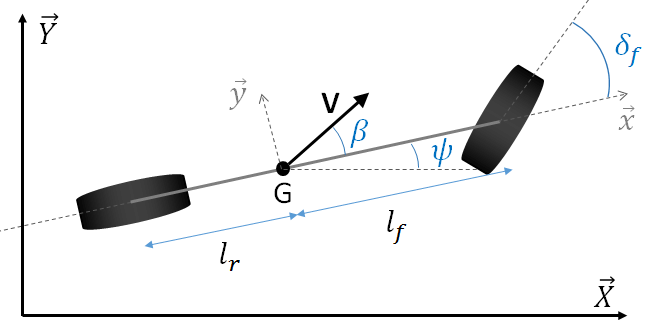
\includegraphics[width=0.5\linewidth]{images/kinematic-bicycle.png}
  \caption[Kinematikai bicikli modell]{Kinematikai bicikli modell \cite{polack2017kinematicBicycleModel}}
  \label{fig:kinematic-bicycle}
\end{figure}

A modellből számunkra fontos megállapítás, hogy a kormány elfordulása, a kerék elfordulása és az autó kanyarodásának pillanatnyi görbülete egyértelmű megfeleltetésben állnak egymással. Az autó kanyarodását két mennyiséggel, a kanyarodás sugarával $(r(t))$ és a görbülettel $(\kappa(t))$ szoktuk jellemezni. $r(t)$ megadja, hogy a jármű mekkora sugarú köríven menne körbe, ha a kerékszög nem változna. A két mennyiség között inverz reláció áll fent: $$r(t) = \frac{1}{\kappa(t)}.$$

Mivel a dinamikai komplexitással az útvonaltervezés csak a megszorítások szintjén foglalkozik, a kinematikai modell legfontosabb paraméterei a minimális kanyarodási sugár $(r_{min})$ és az ennek megfelelő maximális görbület $\left(\kappa_{max} = \frac{1}{r_{min}}\right)$.

\section{Szabadtéri útvonaltervezés}
\textit{Szabadtéri útvonaltervezés} problémának nevezzük, amikor a környezet üres ($\mathcal{E}=\varnothing$), azaz nincsenek akadályok, melyeket ki kéne kerülnünk. Ez önmagában is egy bonyolult optimalizációs feladat lenne, azonban több matematikus munkájának köszönhetően ismerünk analitikus megoldásokat néhány egyszerűbb járműmodellre. Ezen modellek nem foglalják magukba a jármű teljes dinamikai komplexitását, azonban jól közelítik azt alacsony sebességű manővereknél, mint a parkolás.

Egy fontos, jól alkalmazható eredmény a \textit{Reeds--Shepp-útvonal} \cite{reeds1990optimal}. A szerzők egy olyan járművet feltételeztek, mely előre és hátra is azonos költséggel tud közlekedni és a Dubins-autóhoz hasonlóan kanyarodási görbületben limitált. A cikk szerint egy ilyen autó legrövidebb útvonala két pont között az előbb említett C és S primitívekből, illetve irányváltásokból áll és legfeljebb $5$ primitívet és $2$ irányváltást tartalmazhat. A szerzők itt is megadják hogyan lehet analitikusan kiszámítani ezeket az útvonaltípusokat.

Fontos megjegyezni, hogy az útvonalak nem pontonként folytonosak. Egymáshoz közeli célkonfigurációkhoz vezető legrövidebb útvonalak gyakran más mozgási primitíveket tartalmaznak. Ezt szemlélteti \aref{fig:RS-not-pointwise-cont}. ábra.

% hasonló RS feladatok - különböző útvonalak
\begin{figure}[ht] 
    \centering
    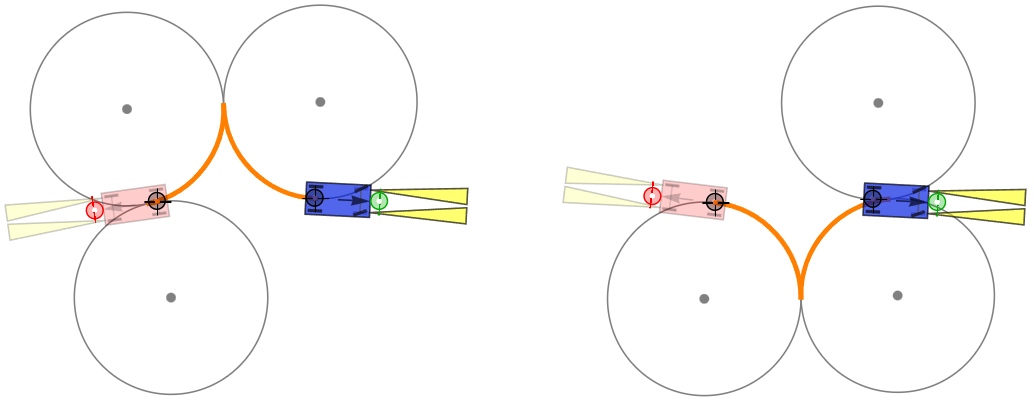
\includegraphics[width=0.9\linewidth]{images/RS-not-pointwise-cont.png}
    \caption[Reeds--Shepp útvonalak nem pontonként folytonosak]{Egymáshoz közeli célkonfigurációkhoz vezető legrövidebb Reeds--Shepp útvonalak lehetnek nagyon különbözők \cite{BernardiniBeckerRSDemonstration}}
    \label{fig:RS-not-pointwise-cont}
\end{figure}

\section{Útvonaltervező algoritmusok}
% Problémafelvetés
Az útvonaltervező algoritmus feladata a bemeneti és kimeneti követelmények figyelembe vételével a környezet felfedezése és egy megfelelő útvonal megtalálása a kiinduló- és a célállapot között. Az általános célú útvonaltervező algoritmusokat két nagyobb csoportra bonthatjuk \cite{gonzalez2015review}. Az egyik a gráfkeresés alapú tervezők, mint a Hibrid A* és változatai. A másik nagy csoport a mintavételezés alapú tervezők, mint az RRT* és variánsai.

\subsection{A* algoritmus}
Az A* algoritmus egy gráfkeresésen alapuló útvonaltervező algoritmus. Az útvonaltervezés során gyakran implicit gráfokat készítünk a paramétertérben, és ezen futtatjuk a tervezőt. Rengeteg variánsa és kiegészítése létezik, melyet \citeauthor{paliwal2023AStarSurvey} jól összefoglal összehasonlító tanulmányában \cite{paliwal2023AStarSurvey}.

% Variánsok
Az algoritmusnak sok variánsa létezik, melyek mind az alap algoritmushoz tesznek hozzá valamit. Ezen variánsok ötletei általában szabadon kombinálhatók egymással \cite{jiang2021analysisIDAStar, reinefeld2002enhancedIDAStar, ammar2024enhancedRelaxedAStar, whangbo2007efficientBidirectionalAStar, koenig2005fastReplanningDStarLite}.

\section{Sima útvonal létrehozása}

Az útvonaltervezés problémája felfogható egy numerikus optimalizációs feladatként is. Ez a megközelítés általában akkor használatos, ha nagy sebesség mellett szeretnénk sima útvonalat tervezni \cite{gonzalez2015review}. A globális tervezés problémájának megoldására nem alkalmas, ha több akadályt is ki kell kerülni, ugyanis többszöri újraindítás esetén sem feltétlenül találja meg az optimális útvonalat.

% Lokális optimalizáció útvonalsimításra
Az optimalizációt érdemes felhasználni az útvonal \textit{lokális simítására} \cite{dolgov2008hybridAstar}. Ezzel elérhetjük, hogy azokon a helyeken, ahol az útvonal körül van szabad hely, simább manővert alakítsunk ki. Ilyenkor az útvonal hosszabb lesz, viszont a simasága miatt a kontroller dinamikusabban tudja  végrehajtani. Az optimalizációban:
\begin{itemize}
  \item minimalizáljuk az útvonal hosszát,
  \item minimalizáljuk a görbületet, és
  \item maximalizáljuk a távolságot az akadályoktól.
\end{itemize}
A görbületre és akadálytávolságra vonatkozó esetekben a célfüggvény jobban bünteti a limitek, pontosabban az akadályok és a görbületi korlátok megközelítését.

\section{Néhány tervezett útvonal}

\begin{figure}[ht]
    \centering
    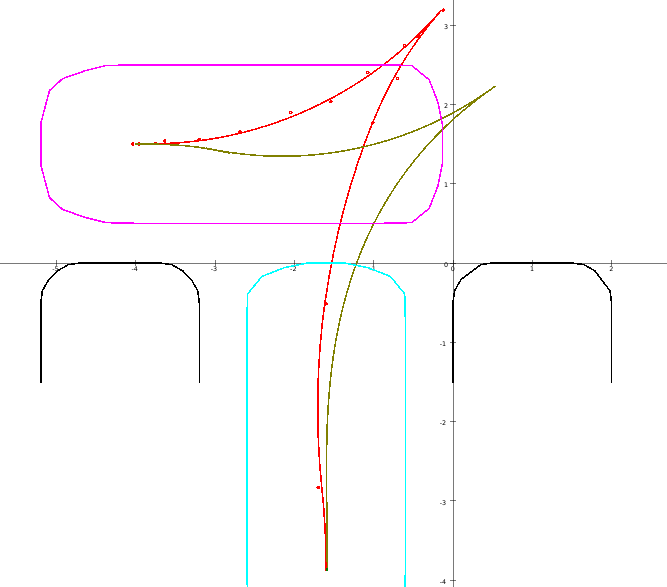
\includegraphics[width=0.5\linewidth]{images/scenes/ISO-cross.png}
    \caption{ISO 20900:2023 merőleges parkolás eset}
    \label{fig:ISO-cross}
\end{figure}

\begin{figure}[ht]
    \centering
    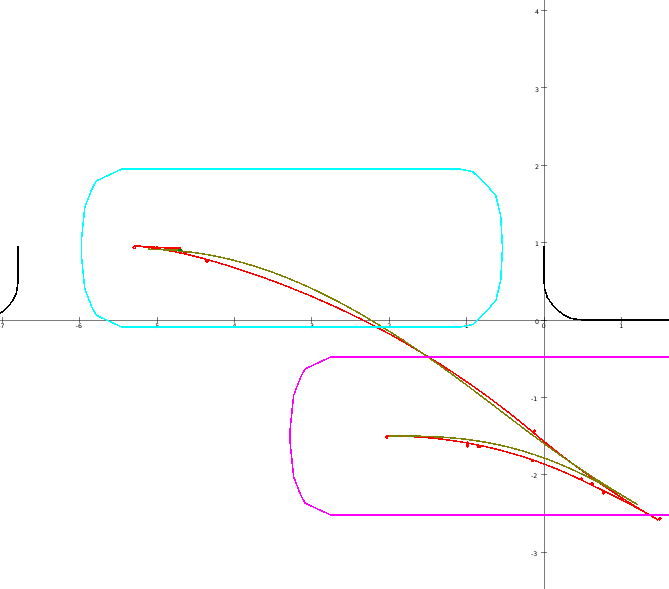
\includegraphics[width=0.5\linewidth]{images/scenes/ISO-parallel.png}
    \caption{ISO 20900:2023 párhuzamos parkolás eset}
    \label{fig:ISO-parallel}
\end{figure}

\begin{figure}[ht]
    \centering
    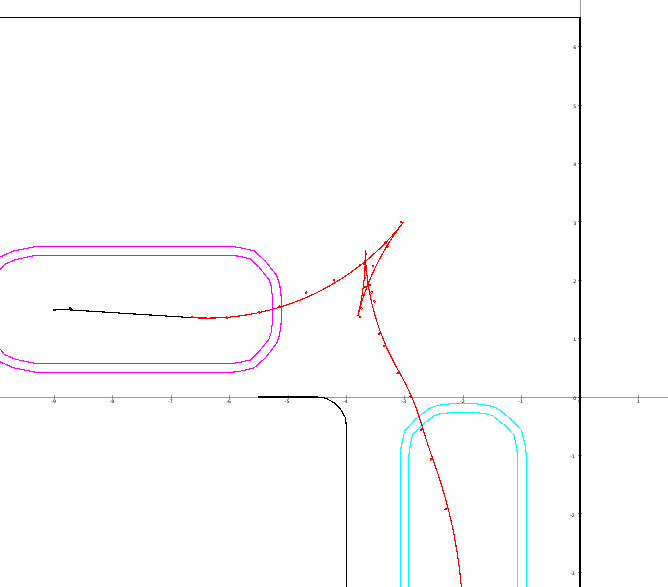
\includegraphics[width=0.45\linewidth]{images/scenes/lastSlot.png}
    \hspace{1em}
    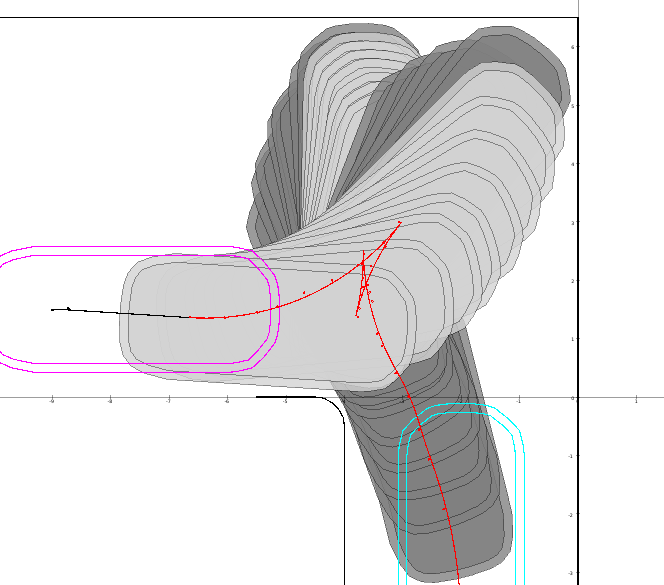
\includegraphics[width=0.45\linewidth]{images/scenes/lastSlot-contour.png}
    \caption{Utolsó helyre parkolás esete egy parkolóházban}
    \label{fig:spec-lastSlot}
\end{figure}




\clearpage
\printbibliography[title=Bibliográfia]

\end{document}
